\chapter{Quickstart}\indexmain{quickstart}\indexmain{example}

In this chapter we'll build a \GrG\ system from scratch.
You should have read already Chapter~\ref{chp:intro} and Chapter~\ref{chp:overview} to have a glimpse of the \GrG\ system and its components.
We will use \GrG\ to construct non-deterministic state machines.
We further show some actual graph rewriting by removing $\varepsilon$-transitions from our state machines.
This chapter is mostly about the \GrG\ look and feel; please take a look at the succeeding chapters for comprehensive specifications.


%%%%%%%%%%%%%%%%%%%%%%%%%%%%%%%%%%%%%%%%%%%%%%%%%%%%%%%%%%%%%%%%%%%%%%%%%%%%%%%%%%%%%%%%%%%%%%%%
\section{Downloading \& Installing}
If you are reading this document, you probably did already download the \GrG\ software from our website (\url{http://www.grgen.net}).
Make sure you have the following system requirements installed and available in the search path:
\begin{itemize}
	\item Java 1.5 or above
	\item Mono 1.2.3 or above / Microsoft .NET 2.0 or above
\end{itemize}

\noindent{\bf If you're using Linux:}
Unpack the package to a directory of your choice, for example into \texttt{/opt/grgen}:
\begin{bash}
mkdir /opt/grgen
tar xvfj GrGenNET-V1_3_1-2007-12-06.tar.bz2
mv GrGenNET-V1_3_1-2007-12-06/* /opt/grgen/
rmdir GrGenNET-V1_3_1-2007-12-06
\end{bash}
Add the \texttt{/opt/grgen/bin} directory to your search paths, for instance if you use \texttt{bash} add a line to your \texttt{/home/.profile} file.
\begin{bash}
export PATH=/opt/grgen/bin:$PATH
\end{bash}
Furthermore we create a directory for our \GrG\ data, for instance by \texttt{mkdir /home/grgen}.

\vspace{2mm}
\noindent{\bf If you're using Microsoft Windows:}
Extract the .zip archive to a directory of your choice and add the \texttt{bin} subdirectory to your search path via \emph{control panel} $\rightarrow$ \emph{system properties} / environment variables.
Execute the \GrG\ assemblies from a command line window (\emph{Start} $\rightarrow$ \emph{Run...} $\rightarrow$ \texttt{cmd}).
For MS .NET the \texttt{mono} prefix is neither applicable nor needed.

\begin{note}
You might be interested in the syntax highlighting specifications of the \GrG-languages supplied for the vim, Emacs, and Notepad++ editors in the \texttt{syntaxhighlighting} subdirectory.
\end{note}


%%%%%%%%%%%%%%%%%%%%%%%%%%%%%%%%%%%%%%%%%%%%%%%%%%%%%%%%%%%%%%%%%%%%%%%%%%%%%%%%%%%%%%%%%%%%%%%%
\section{Creating a Graph Model}
In the directory \texttt{/home/grgen} we create a text file \texttt{StateMachine.gm} that contains the graph meta model for our state machine\footnote{You'll find the source code of this quick start example shipped with the \GrG\ package in the \texttt{examples/FiniteStateMachine/} directory.}.
By graph meta model we mean a set of node types and edge types which are available for building state machine graphs (see Chapter~\ref{chapmodellang}).
Figure \ref{fig:quick:mm} shows the meta model.
\begin{figure}[htbp]
    \centering
    \begin{grgen}
node class State {
    id: int;
}

abstract node class SpecialState extends State;
node class StartState extends SpecialState;
node class FinalState extends SpecialState;
node class StartFinalState extends StartState, FinalState;

edge class Transition {
    Trigger: string;
}

const edge class EpsilonTransition extends Transition;
    \end{grgen}
    \caption{Meta Model for State Machines}
    \label{fig:quick:mm}
\end{figure}
What have we done?
You can see two base types, \texttt{State} for state nodes and \texttt{Transition} for transition edges that will connect the state nodes.
\texttt{State} has an integer attribute \texttt{id} and \texttt{Transition} has a string attribute \texttt{Trigger} which indicates the character sequence for switching from the source state node to the destination state node.
For the rest of the types we use inheritance (keyword \texttt{extends}) which works more or less like inheritance in object oriented languages.
Accordingly the \texttt{abstract} modifier for \texttt{SpecialState} means that you cannot create a node of that precise type, but you might create nodes of non-abstract subtypes.
As you can see \GrG\ supports multiple inheritance, and with \texttt{StartFinalState} we have constructed a ``diamond'' type hierarchy.


%%%%%%%%%%%%%%%%%%%%%%%%%%%%%%%%%%%%%%%%%%%%%%%%%%%%%%%%%%%%%%%%%%%%%%%%%%%%%%%%%%%%%%%%%%%%%%%%
\section{Creating Graphs}
\label{sct:quick:create}
Let's test our graph meta model by creating a state machine graph.
We will use the \GrShell\ (see Chapter~\ref{chapgrshell}) and---for visualization---\yComp.
To get everything working we need a rule set file, too.
For the moment we just create an almost empty file \texttt{removeEpsilons.grg} in the \texttt{/home/grgen} directory, containing only the line
\begin{grgen}
#using "StateMachine.gm"
\end{grgen}
Now, we could start by launching the \GrShell\ and typing the commands interactively.
This is, however, in most of the cases not the preferred way.
We rather create a \GrShell\ script, say \texttt{removeEpsilons.grs}, in the \texttt{/home/grgen} directory.
Figure \ref{fig:quick:shell} shows this script.
Run the script by executing \texttt{grshell removeEpsilons.grs}.
The first time you execute the script, it might take a while because \GrG\ has to compile the meta model and the rule set into .NET assemblies.
\begin{figure}[htbp]
    \centering
    \begin{grgen}
new graph removeEpsilons "StateMachineGraph"

new :StartState($=S, id=0)
new :FinalState($=F, id=3)
new :State($="1", id=1)
new :State($="2", id=2)
new @(S)-:Transition(Trigger="a")-> @("1")
new @("1")-:Transition(Trigger="b")-> @("2")
new @("2")-:Transition(Trigger="c")-> @(F)
new @(S)-:EpsilonTransition-> @("2")
new @("1")-:EpsilonTransition-> @(F)
new @(S)-:EpsilonTransition-> @(F)

show graph ycomp
    \end{grgen}
    \caption{Constructing a state machine graph in \GrShell}
    \label{fig:quick:shell}
\end{figure}
The graph viewer \yComp\ opens and after clicking the blue ``layout graph'' button on the very right side of the button bar, you get a window similar to figure \ref{fig:quick:ycomp} (see also Section~\ref{tools:ycomp}).
\begin{figure}[htbp]
	\centering
	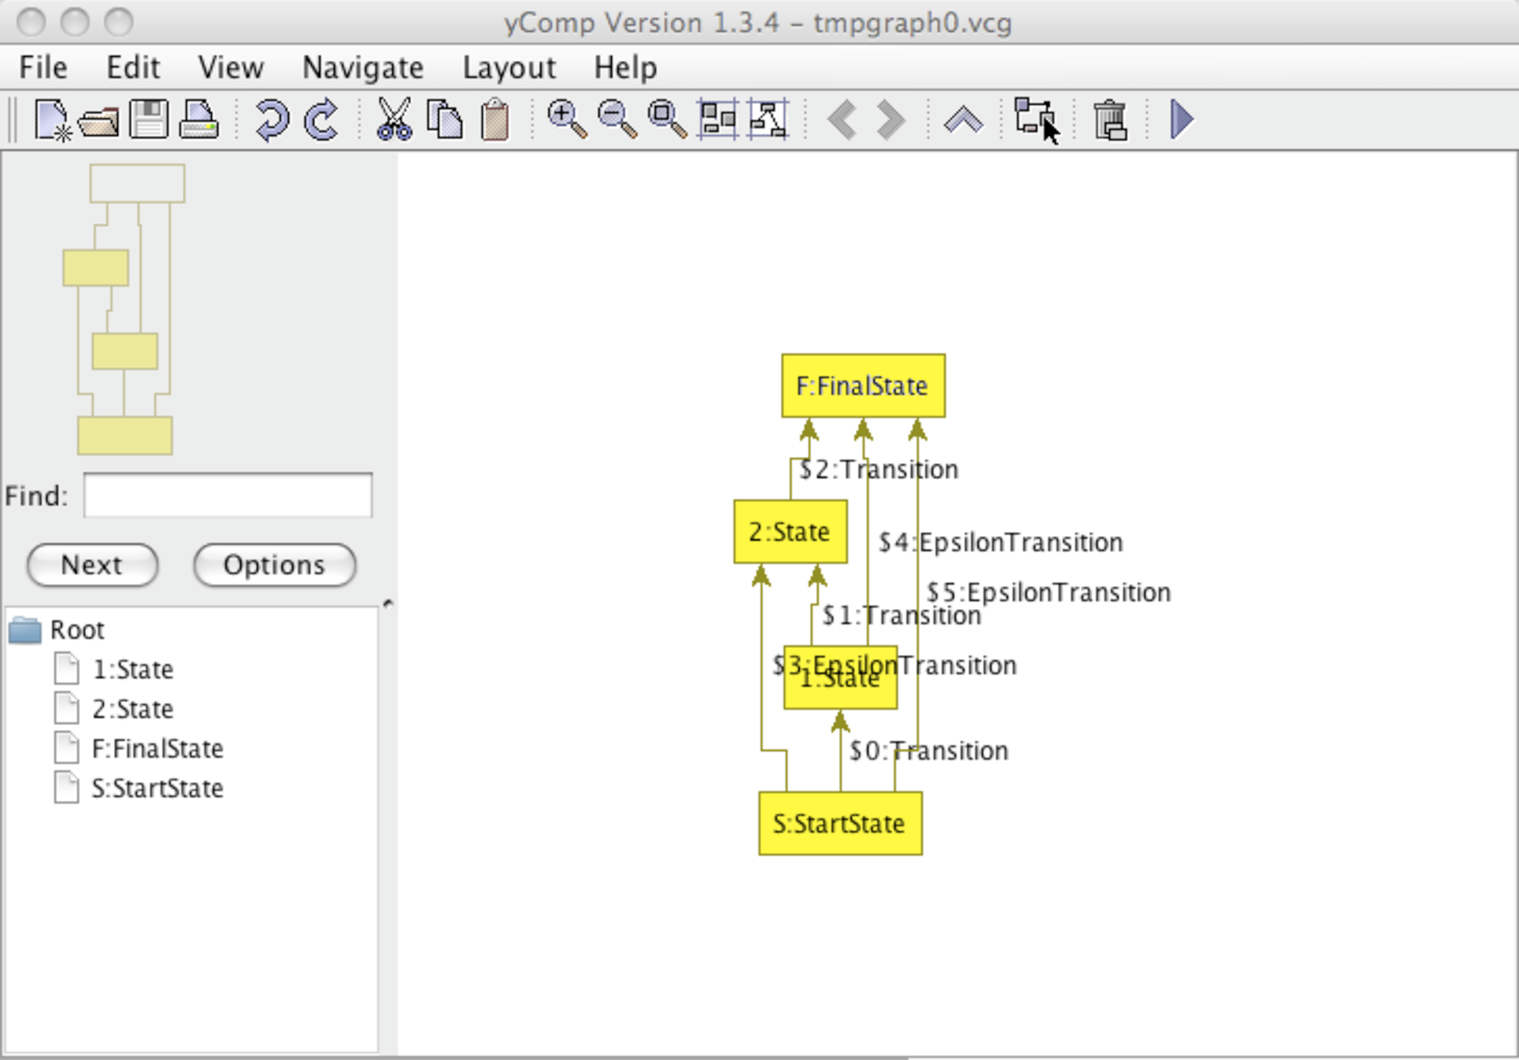
\includegraphics[width=0.8\linewidth]{fig/quickycomp}
	\caption{A first state machine}
	\label{fig:quick:ycomp}
\end{figure}
The graph looks still a bit confusing.
In fact it is quite normal that \yComp's automatic layout algorithm needs manual adjustments.
Quit \yComp\ and exit the \GrShell\ by typing \texttt{exit}.

This script starts with creating an empty graph of the meta model \texttt{StateMachine} (which is referenced by the rule set \texttt{removeEpsilons.grg}) with the name \texttt{StateMachineGraph}.
Thereafter we create nodes and edges.
The colon notation indicates a node or edge type.
Also note the inplace-arrow notation for edges (\texttt{-Edge->} resp.\ \texttt{-:EdgeType->}).
As you can see, attributes of graph elements can be set during creation with a call-like syntax.
\makeatletter
The \texttt{\$} and \texttt{@} notation is due to the fact that we have two kinds of ``names'' in the \GrShell.
Namely we have \emph{global variables}---which we did not use, no global variable is explicitly defined in this script---and \emph{persistent names} that denote a specific graph element.
Persistent names are set by \texttt{\$=Identifier} on creation and they are accessed by \texttt{@(Identifier)}.
\makeatother
The quote chars around \texttt{"1"} and \texttt{"2"} are used to type these characters as (identifier) strings rather than numbers.


%%%%%%%%%%%%%%%%%%%%%%%%%%%%%%%%%%%%%%%%%%%%%%%%%%%%%%%%%%%%%%%%%%%%%%%%%%%%%%%%%%%%%%%%%%%%%%%%
\section{The Rewrite Rules}
We will now add the real rewrite rules to the rule set file \texttt{removeEpsilons.grg}.
The idea is to ``forward'' the $\varepsilon$-transitions one after another, i.e.\ if we have a pattern like \texttt{a:State -EpsilonTransition-> b:State -e:Transition-> c:State} we forward to \texttt{a -e-> c}.
After all such transitions are forwarded we can remove the $\varepsilon$-transitions alltogether.
The complete rule set is shown in figure \ref{fig:quick:ruleset}.
See Chapter~\ref{chaprulelang} for the rule set language reference.
\begin{figure}[htbp]
	\centering
	\begin{grgen}
#using "StateMachine.gm"

test checkStartState {
    x:StartState;
    negative {
        x;
        y:StartState;
    }
}

test checkDoublettes {
    negative {
        x:State -e:Transition-> y:State;
        hom(x,y);
        x -doublette:Transition-> y;
        if {typeof(doublette) == typeof(e);}
        if { ((typeof(e) == EpsilonTransition) || (e.Trigger == doublette.Trigger)); }
    }
}

rule forwardTransition {
    x:State -:EpsilonTransition-> y:State -e:Transition-> z:State;
    hom(x,y,z);
    negative {
        x -exists:Transition-> z;
        if {typeof(exists) == typeof(e);}
        if { ((typeof(e) == EpsilonTransition) || (e.Trigger == exists.Trigger)); }
    }
    modify {
        x -forward:typeof(e)-> z;
        eval {forward.Trigger = e.Trigger;}
    }
}

rule addStartFinalState {
    x:StartState -:EpsilonTransition-> :FinalState;
    modify {
        y:StartFinalState<x>;
        emit("Start state (", x.id, ") mutated into a start-and-final state");
    }
}

rule addFinalState {
    x:State -:EpsilonTransition-> :FinalState;
    if {typeof(x) < SpecialState;}
    modify {
        y:FinalState<x>;
    }
}

rule removeEpsilonTransition {
    -:EpsilonTransition->;
    replace {}
}
	\end{grgen}
	\caption{Rule set for removing $\varepsilon$-transitions}
	\label{fig:quick:ruleset}
\end{figure}

In detail: The rule set file consists of a number of rules and tests, each of them bearing a name, like \texttt{forwardTransition}.
Rules contain a pattern expressed as several semicolon-separated pattern statements and a modify part or a rewrite part.
Tests contain only a pattern; they are used to check for a certain pattern without doing any rewrite operation.
If a rule is applied, \GrG\ tries to find the pattern within a host graph, for instance within the graph we created in Section~\ref{sct:quick:create}.
Of course there could be several matches for a pattern---\GrG\ will choose one of them arbitrarily.

Figure \ref{fig:quick:ruleset} also shows the syntax \texttt{x:NodeType} for nodes and \texttt{-e:EdgeType->} for Edges, which we have already seen in Section~\ref{sct:quick:create}.
There are also statements like \texttt{:FinalState} or \texttt{-:EpsilonTransistion->}, i.e.\ we are searching for a node of type \texttt{FinalState} resp.\ an edge of type \texttt{EpsilonTransition}, but we are not assigning these graph elements to a name (like \texttt{x} or \texttt{e} above).
Defining of names is a key concept of the \GrG\ rule sets: names work as connection points between several pattern statements and between the pattern and the replace / modify part.
As a rule of thumb: If you want to do something with your found graph element, define a name; otherwise an anonymous graph element will do fine.
Also have a look at example \ref{ex:somegraphlets} on page \pageref{ex:somegraphlets} for additional pattern specifications.
The difference between a replace part and a modify part is that a replace part deletes every graph element of the pattern which is not explicitly mentioned within its body.
The modify part, in contrast, deletes nothing (by default), but just adds or adjusts graph elements.
However, the modify part allows for \emph{explicit} deletion of graph elements by using the \texttt{delete} statement.

What else can we do?
We have negative application conditions (NACs), expressed by \texttt{negative \{\dots\}}; they prevent rules to be applied if the negative pattern is found.
We also have attribute conditions, expressed by \texttt{if \{\dots\}}; a rule is only applicable if all such conditions yield true.
Note, the dot notation to access attributes (as in \texttt{e.Trigger}).
The \texttt{emit} statement prints a string to \texttt{stdout}.
The \texttt{hom(x,y)} and \texttt{hom(x,y,z)} statements mean ``match the embraced nodes homomorphically'', i.e.\ they can (but they don't have to) actually be matched to the same node within the host graph.
The \texttt{eval \{\dots\}} statement is used to recalculate attributes of graph elements.
Have a look at the statement \texttt{y:StartFinalState<x>} in \texttt{addStartFinalState}: we \emph{retype} the node \texttt{x}.
That means the newly created node \texttt{y} is actually the node \texttt{x} (including its incident edges and attribute values) except for the node type which is changed to \texttt{StartFinalState}.
Imagine retyping as a kind of a type cast.

The created rewrite rules might be considered as rewrite primitives.
In order to implement more complex functionality, we will compose a sequence of rewrite rules out of them.
For instance we don't want to forward just one $\varepsilon$-transition as \texttt{forwardTransition} would do; we want to forward them all.
Such a rule composing is called \emph{graph rewrite sequence} (see Chapter~\ref{cha:xgrs}).
We add the following line to our shell script \texttt{removeEpsilons.grs}:
\begin{grgen}
debug exec checkStartState && !checkDoublettes && (forwardTransition* | addStartFinalState | addFinalState* | removeEpsilonTransition* | true)
\end{grgen}
This looks like a boolean expression and in fact it behaves similar.
The whole expression is evaluated from left to right.
A rule is successfully evaluated if a match could be found.
The negation operator \texttt{!} toggles the result.
We first check for a valid state machine, i.e.\ if the host graph contains exactly one start state and no redundant transitions.
Thereafter we do the actual rewriting.
These three steps are connected by lazy-evaluation-ands (\texttt{\&\&}), i.e.\ if one of them fails the evaluation will be canceled.
We continue with disjunctively connected rules (by \texttt{|}).
The eager operator causes all rules to get executed, but only one must find a match for success; the final \texttt{true} ensures overall success.
The \texttt{*} is used to apply the rule repeatedly as long as a match can be found.
This includes applying the rule zero times.
Even in this case \texttt{Rule*} is still successful.


%%%%%%%%%%%%%%%%%%%%%%%%%%%%%%%%%%%%%%%%%%%%%%%%%%%%%%%%%%%%%%%%%%%%%%%%%%%%%%%%%%%%%%%%%%%%%%%%
\section{Debugging and Output}
If you execute the modified \GrShell\ script, \GrG\ starts its debugger.
This way you can follow the evaluation of the graph rewrite sequence step by step in \yComp.
Just play around with the keys \texttt{d}, \texttt{s}, and \texttt{r} in \GrShell: the \texttt{d} key lets you follow a single rewrite operation in multiple steps; the \texttt{s} key jumps to the next rule; and the \texttt{r} key runs to the end of the graph rewrite sequence.
Finally you should get a graph like the one in figure \ref{fig:quick:final}
\begin{figure}[htbp]
	\centering
	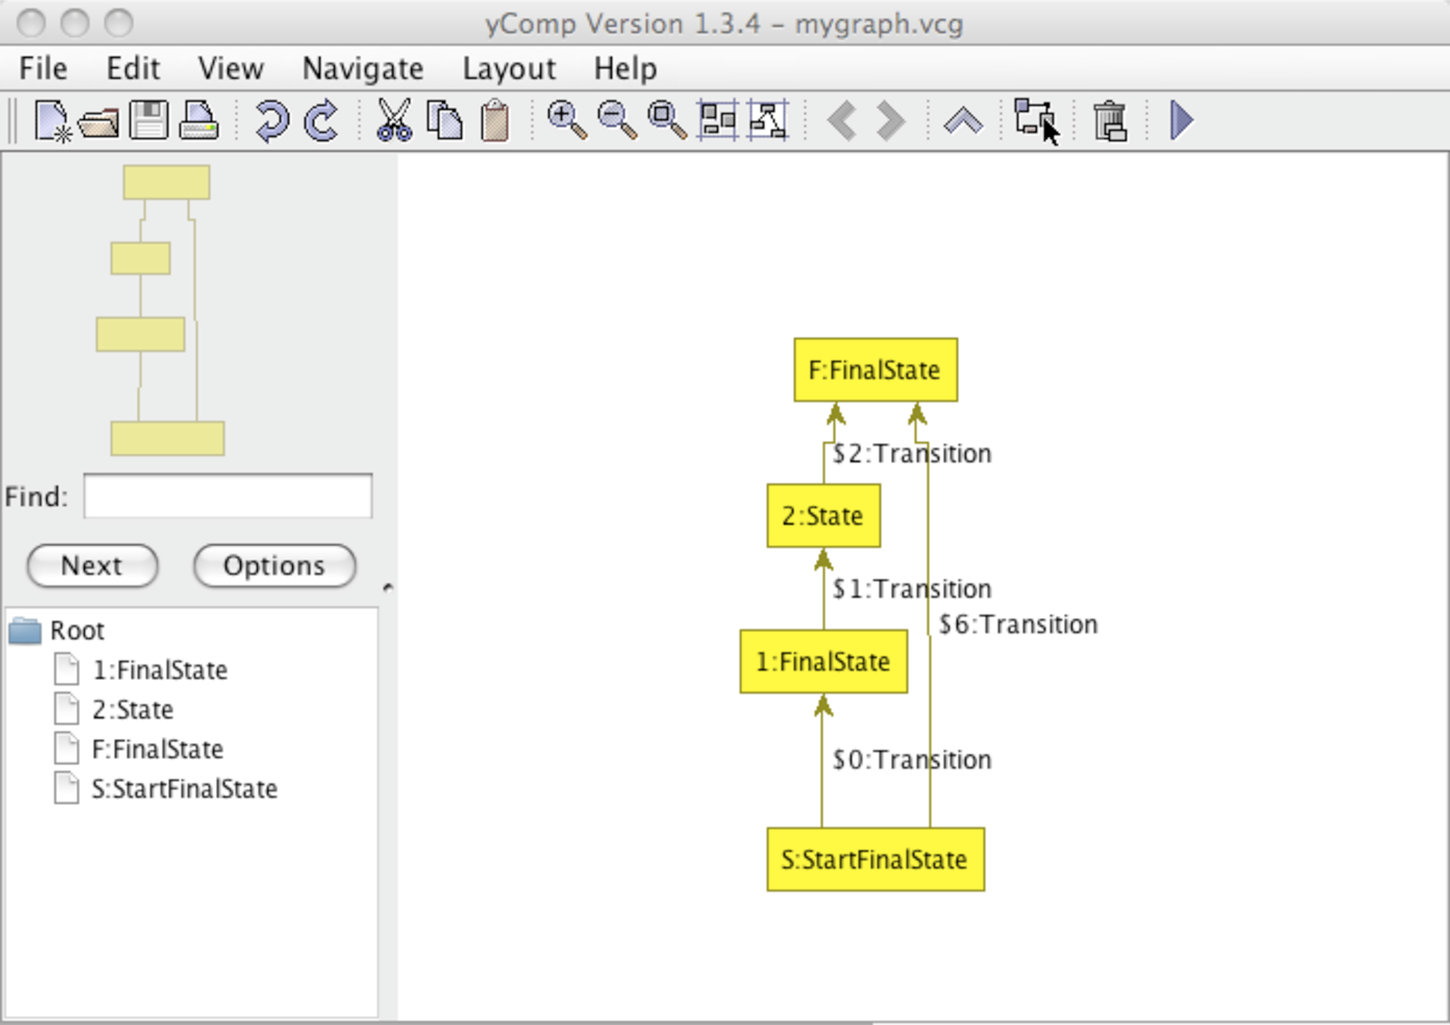
\includegraphics[width=0.8\linewidth]{fig/quickfinal}
	\caption{A state machine without $\varepsilon$-transitions}
	\label{fig:quick:final}
\end{figure}

If everything is working fine you can delete the \texttt{debug} keyword in front of \texttt{exec}.
Maybe you want to save a visualization of the resulting graph.
This is possible by typing \texttt{dump graph mygraph.vcg} in \GrShell,
writing \texttt{mygraph.vcg} into the current directory in VCG format readable by \yComp.
Feel free to browse the \texttt{examples} folder shiped with \GrG\ ;
esp. the succession of examples in \texttt{FiniteStateMachine} and \texttt{ProgramGraphs}
is recommended to have a look at, they give an overview of the capabilities of the software.

